\documentclass[a4paper]{scrartcl}
\usepackage[utf8]{inputenc}
\usepackage{amsmath}
\usepackage{amssymb}
\usepackage{amsopn}
\usepackage{enumitem}
\usepackage{graphicx}
\usepackage{placeins}

\newcommand\norm[1]{\left\lVert #1 \right\rVert}
\newcommand\abs[1]{\left| #1 \right|}
\newcommand\paren[1]{\left( #1 \right)}
\newcommand\brak[1]{\left[ #1 \right]}
\newcommand\curly[1]{\left\{ #1 \right\}}
\newcommand\innerprod[1]{\left\langle #1 \right\rangle}
\newcommand\N{\mathbb N}
\newcommand\Z{\mathbb Z}
\newcommand\F{\mathbb F}
\newcommand\cP{\mathcal P}
\newcommand\cC{\mathcal C}
\newcommand\cK{\mathcal K}
\renewcommand\mod{\hspace*{0.4em}\mathrm{mod}\hspace*{0.2em}}

\DeclareMathOperator\ess{ess}
\DeclareMathOperator\supp{supp}
\DeclareMathOperator\sinc{sinc}
\DeclareMathOperator\sgn{sgn}
\newcommand\df{\:\mathrm d}
\setlength\parindent{0em}
\setlength\parskip{0.75em}

\title{Cryptography}
\subtitle{SS 2017}

\begin{document}

\maketitle
\thispagestyle{empty}
\newpage

\tableofcontents
\newpage


\section{Historical examples}

\subsection{Encryption and decryption functions}

Define\begin{itemize}
    \item $\cP$ the set of plaintexts
    \item $\cC$ the set of ciphertexts
    \item $f: \cP \rightarrow \cC$, $f$ injective the encryption function
    \item $g: \cC \rightarrow \cP,\;g=f^{-1}$ the decryption function
\end{itemize}

\subsection{Substitution / permutation ciphers}

Message unit is one symbol $\in \cP = \cC = A := \{a,\hdots,z\}$,
$f$ is any permutation $A \rightarrow A$. Break using letter frequency.

\subsubsection{Shift ciphers}

Special case of substitution ciphers: $A = \Z_N$, fix key $K\in\mathbb K_N$,
$f: m\mapsto (m + K)\mod N$. Classical example: \textit{Ceasar cipher} with $K=3$

\subsubsection{Vigen\`ere cipher}

Message unit is a sequence of $k$ symbols, i.e. $\cP = \cC = A^k = \Z_N^k$,
fix key $(K_1,\hdots,K_N)$, $f: (m_1,\hdots)\mapsto((m_1+K_1)\mod N, \hdots)$

\subsubsection{Affine / Hill ciphers}

Generalization of shift / Vigen\`erre ciphers. For fixed $k$, choose keys $a\in\Z^{k\times k},
b\in\Z^k$, $a$ invertible and define $f: m\mapsto am+b$ and its inverse $g: c\mapsto a^{-1}(c-b)$
with matrix operations modulo $N$. 

\newpage
\section{Encryption with keys}

\textit{Keyed cryptosystem}: Define\begin{itemize}
    \item $\cK$ the key space
    \item $f: \cP\times\cK\rightarrow\cC$ with the
        \textit{encryption key} $k$ the keyed encryption function 
    \item $g: \cC\times\cK\rightarrow\cP,\;g(f(m,k),k')=m$ with the
        \textit{decryption key} $k'$ the keyed decryption function 
\end{itemize}

Where convenient, write $f(k, \cdot)$ as $f_k$ and $g(k',\cdot)$ as $g_k'$.

\subsection{Symmetric vs. public key encryption}

Encryption and decryption maps $f, g$ are public and efficiently computable (Kerkhoff).

\begin{itemize}
    \item In \textit{symmetric key} encryption $k=k'$ and $k$ is secret. Fast. Example: Ceasar.

    \item In \textit{public key} encryption $k$ is public and $k'$ is secret with $k\neq k'$.
        Usually slower to compute than symmetric key encryption.

    \item \textit{Mixed encryption} is an efficient combination: A \textit{session key} is
        transferred using public key cryptography and used to encrypt data with a fast symmetric
        key cryptosystem
\end{itemize}

\subsection{Mixed Encryption}

\begin{enumerate}
    \item Public key cryptosystem generates \textit{session key} (slow)
    \item Content is encrypted via symmetric cryptosystem (fast)
\end{enumerate}

\subsection{Block ciphers}

A \textit{block cipher} of (fixed) \textit{block length} $n$ is defined by encryption and decryption functions
\[f_k,g_k:A^n\rightarrow A^n,\quad g_k=f_k^{-1}\]

\begin{itemize}
    \item \textbf{Substitution cipher} (S-box): Let $\sigma: A\rightarrow A$ bijective and set
        \[f(a_1,\hdots,a_n) := (\sigma(a_1),\hdots,\sigma(a_n))\]
    \item \textbf{Transposition cipher}: Let $\tau: \{1,\hdots,n\} \rightarrow \{1,\hdots,n\}$ and set
        \[f(a_1,\hdots,a_n) := (a_{\tau(1)},\hdots,a_{\tau(n)})\]
    \item \textbf{Iterated cipher}: Multiple iterations (\textit{rounds}) of substitutions and
        transpositions with different \textit{round keys} generated from the master key.
\end{itemize}

\subsection{Stream ciphers}

Use a fast \textit{keystream generator} $g_K$ for a master key $K$ to generate a sequence of
keys $k_0, k_1,\hdots$.

Encrypt message via \[f_K(m) = (f_{k_1}(m_1), f_{k_2}(m_2),\hdots)\]

\subsubsection{Affine stream ciphers}

Keystream generator ($a\in\Z^*_N, b\in\Z_N$):
\[g: \Z_N\rightarrow \Z_N,\quad x\mapsto ax+b\]
generate from given $k_0$
\[k_{i+1}=g(k_i)\]
and encrypt via
\[c_i = m_i + k_i \mod n\]

\textbf{Maximal period:} If $N=2^m$, the maximal period of $2^m$
is achieved iff $a\equiv1\mod4$ and $b$ is odd.

\subsection{Linear Feedback Shift Registers}

??? Lecure week 2 page 15

\section{Data Encryption Standard}

\subsection{Feistel cipher}

Given a master key $K$ and a length $t$ block cipher $f_k:\{0,1\}^t\rightarrow\{0,1\}^t$,
construct \begin{itemize}
    \item $r$ round keys $k_1,\hdots,k_r$
    \item a length $2t$ block cipher $F_k:\{0,1\}^{2t}\rightarrow\{0,1\}^{2t}$
\end{itemize}

Set $F_K(a_0,b_0) := (b_r, a_r)$, encrypt with
\[(a_i,b_i):=(b_{i-1}, a_{i-1}\oplus f_{k_i}(b_{i-1}))\]
and decrypt via
\[(b_{i-1},a_{i-1}) = (a_i,b_i\oplus f_{k_i}(a_i))\]

\begin{figure}
    \centering
    \includegraphics[scale=0.35]{images/feistel.png}
    \caption{Feistel network}
\end{figure}

\subsection{DES structure}

DES uses 64 bit keys with 8 parity bits, e.g. 56 bits of security.

\subsubsection{Transposition maps}

DES has a fixed initial (bijective) permutation $\sigma: \{0,1\}^{64} \rightarrow \{0,1\}^{64}$.
\begin{enumerate}
    \item Apply $f_\sigma$
    \item Apply 16 round Feistel chipher
    \item Apply $f_\sigma^{-1}$
\end{enumerate}

\subsubsection{Internal block cipher}

For the Feistel chipher, the 64-bit block is split into two 32-bit blocks which are encrypted
and swapped according to the Feistel rules.

\begin{enumerate}
    \item Expand from $\{0,1\}^{32}$ to $\{0,1\}^{48}$ by duplicating every other bit
    \item XOR the result with the round key as derived by the key schedule
    \item Split 48-bit block into 8 6-bit blocks, then apply a fixed, but different S-box to each
        6-bit block, resulting in 8 4-bit blocks that are combined to a 32-bit output
    \item Permute the 32-bit block using a fixed \textit{P-box}
\end{enumerate}

\begin{figure}
    \centering
    \includegraphics[scale=0.2]{images/des.png}
    \caption{DES internal block cipher}
\end{figure}

\subsubsection{Key schedule}

\begin{enumerate}
    \item Remove parity bits from key to obtain 56 key bits
    \item Split into two 28-bit blocks
    \item For each round key to generate:
    \begin{enumerate}
        \item Left-rotate both 28-bit blocks by one or two bits
        \item Choose 24 bits from each block using a fixed permutation / substitution
            to build a 48 bit round key
    \end{enumerate}
\end{enumerate}

\begin{figure}
    \centering
    \includegraphics[scale=0.5]{images/des-schedule.png}
    \caption{DES key schedule}
\end{figure}

\section{Finite fields}

\textbf{Example:} Prime fields $\F_p$, where $p$ is a prime. Denoted by
$\F_5=\{\overline 0,\overline1,\overline2,\overline3,\overline4\}$.

\textbf{Lemma:} Any finite field $F$ has cardinality $|F|=p^m$, where
$p$ is a prime.

\subsection{Properties of module operations}
\subsubsection{Homomorphism law}

\[(a+b)\mod p = (a \mod p + b \mod p) \mod p\]
\[(a\cdot b)\mod p = (a \mod p \cdot b \mod p) \mod p\]

\subsubsection{Primitive roots}
A \textit{primitive root} modulo $p$ is a number $g$, such that $g^x\mod p$ assumes
all values in $\{1,\hdots,p-1\}$ for suitable $x\in\N$.

\subsubsection{Residue class rings}

For $n\in\N$, the residue class ring $\Z_n = \{\overline0,\overline1,\hdots,\overline{n-1}\}$
is a field iff $n$ is a prime.

\subsection{Binary sequences}

Binary sequences: Polynomials in $\{0,1\}=\F_2[x]$
\begin{itemize}
    \item Addition becomes XOR $\oplus$
    \item Multiplication becomes CLMUL $\otimes$ (carry-less multiplication), i.e. shift-and-xor
        instead of shift-and-add
    \item Division becomes carry-less division $\ominus$, i.e. carry-less long division with
        remainder (mod)
\end{itemize}

\subsubsection{Irreducible binary sequences}

An element $p\in\{0,1\}^*$ is irreducible (``prime''), if there are no $a,b\neq1$ such
that $a\otimes b=p$.

\textbf{Example:} The first irreducible elements are
\[10, 11, 111, 1011, 1101\]
which correspond to the polynomials
\[x,\ x+1,\ x^2+x+1,\ x^3+x+1,\ x^3+x^2+1\]

\subsubsection{Modular arithmetic for binary sequences}

If $p$ is an irreducible polynomial of degree $m$, the residue classes modulo $p$
define the binary field $\F_{2^m}$.

\subsection{Extended Euclidean Algorithm}

For any $a,b\in\N$ there exist $s,t\in\Z$ such that\[\gcd(a,b)=sa+tb\]

\textbf{Start:}
\begin{center}
    \begin{tabular}{cc|cc}
        $-q$ & $r_n$ & $s_n$ & $t_n$ \\ 
        \hline
            & $a$ & 1 & 0 \\
            & $b$ & 0 & 1\\
        \multicolumn{2}{c}{$\hdots$}& \multicolumn{2}{c}{$\hdots$}
    \end{tabular}
\end{center}

\textbf{Step:} Repeat
\begin{enumerate}
    \item Divide $r_k$ by $r_{k-1}$ to get quotient $-q_k$ and remainder $r_{k+1}$
        (note the different indices!). If $r_{k+1} = 0$, finish with
        \[\gcd(a,b)\;=\;r_k\;=\;s_ka+t_kb\]
    \item Calculate $s_{k+1} := s_{k-1}-qs_k$
    \item Calculate $t_{k+1} := t_{k-1}-qt_k$
\end{enumerate}

\subsubsection{Euclid's Lemma}

If $p$ is prime and $a,b\in\N$ with $p\mid ab$, then either $p|a$ or $p|b$.

\subsubsection{Modular inversion}

$\overline a\in\Z_n$ is invertible iff $\gcd(a,n)=1$.

\subsection{Euclidean domains}

The Euclidean algorithm also applies to other \textit{integral domains}, not just $\Z$.

An \textbf{integral domain} is a commutative ring without zero divisors, i.e. where
\[a,b\neq0\;\Rightarrow\;a\cdot b\neq0\]

An \textbf{Euclidean domain} is an integral domain $R$ with a \textit{degree function}
$d: R\rightarrow \N$ where for each $f,g\in R, g\neq0$ there
exists $q,r\in R$ such that \[f\;=qg+r\quad\text{and}\quad d(r)<d(g)\]

Examples:\begin{itemize}
    \item For $R=\Z$, $d = |\cdot|$
    \item For $R=F[x]$ (polynomial), where F is a field, $d=\deg$
\end{itemize}

\section{Advanced Encryption Standard}

128-bit block cipher.

\textbf{Three versions:}
\begin{center}
    \begin{tabular}{c|ccc}
        key length & 128 & 192 & 256 \\
        \hline
        rounds & 10 & 12 & 14
    \end{tabular}
\end{center}

\textbf{Basic Algorithm:}
\begin{enumerate}
    \itemsep-5pt
    \item AddRoundKey
    \item $r-1$ times:
        \vspace*{-5pt}
        \begin{enumerate}[label=\arabic*.]
        \itemsep-5pt
            \item SubBytes
            \item ShiftRows
            \item MixColumns
            \item AddRoundKey
        \end{enumerate}
    \item SubBytes
    \item ShiftRows
    \item AddRoundKey
\end{enumerate}

\FloatBarrier

\subsection{SubBytes}

Use the finite field $\F_{256}\;:=\;\F_2[x]/(x^8+x^4+x^2+x+1)$, which is isomorphic to $(\F_2)^8$,
and define $0^{-1} = 0$.

SubBytes is a non-linear map of the form
\[S:b\mapsto Ab^{-1}+c\]
with fixed $A$ and $c$.

\begin{figure}
    \centering
    \includegraphics[scale=0.25]{images/subbytes.png}
    \caption{SubBytes}
\end{figure}

\subsection{ShiftRows}

ShiftRows views the 128-bit-block as a $4\times4$-Matrix with 8-bit entries,
and computes a new matrix by rotating the $i$th row left by $i-1$ columns.

\begin{figure}
    \centering
    \includegraphics[scale=0.3]{images/shiftrows.png}
    \caption{ShiftRows}
\end{figure}

\subsection{MixColumns}

The $4\times4$-Matrix is split into four columns, which are represented by the polynomial
\[a_3x^3 + a_2x^2 + a_1x + a_0\;\in\;\F_{256}[x]\]
Multiplying it with the fixed polynomial
\[3x^3 + x^2 + x + 2\]
yields the MixColums result which can be written as a linear system
\[\begin{pmatrix}
    b_0\\b_1\\b_2\\b_3
\end{pmatrix}\;=\;\begin{pmatrix}
    2 & 3 & 1 & 1 \\
    1 & 2 & 3 & 1 \\
    1 & 1 & 2 & 3 \\
    3 & 1 & 1 & 2
\end{pmatrix}\begin{pmatrix} 
    a_0\\a_1\\a_2\\a_3
\end{pmatrix}\]
This step is similar to a Hill cipher.

\begin{figure}
    \centering
    \includegraphics[scale=0.25]{images/mixcolumns.png}
    \caption{MixColumns}
\end{figure}

\subsection{AddRoundKey}

In each AddRoundKey step, the 128-bit block is XORed with a 128-bit \textit{Round Key} as
derived from the key schedule.

\subsection{Key Schedule}

Round key $k^{i+1}$ is derived from $k^{i}$ by applying RotWord, SubWord, Rcon and XOR operations
in the order shown in figure \ref{aesschedule}.

The RotWord-SubWord-Rcon block is actually
\[\mathrm{SubWord}(\mathrm{RotWord}(w))\oplus \mathrm{Rcon}(i)\]

\subsubsection{RotWord}

Performs an 8-bit left-rotation of the 32-bit word.
\[(b_0,b_1,b_2,b_3)\mapsto(b_1,b_2,b_3,b_0)\]

\subsubsection{SubWord}

SubBytes (the S-box operation) applied to each byte of the 32-bit word.
\[(b_0,b_1,b_2,b_3)\mapsto(Ab_0^{-1}+c,Ab_1^{-1}+c,Ab_2^{-1}+c,Ab_3^{-1}+c)\]

\subsubsection{Rcon}

Rcon is an exponentiation operation
\[n\mapsto (x^n, 0, 0, 0)\]

\begin{figure}
    \centering
    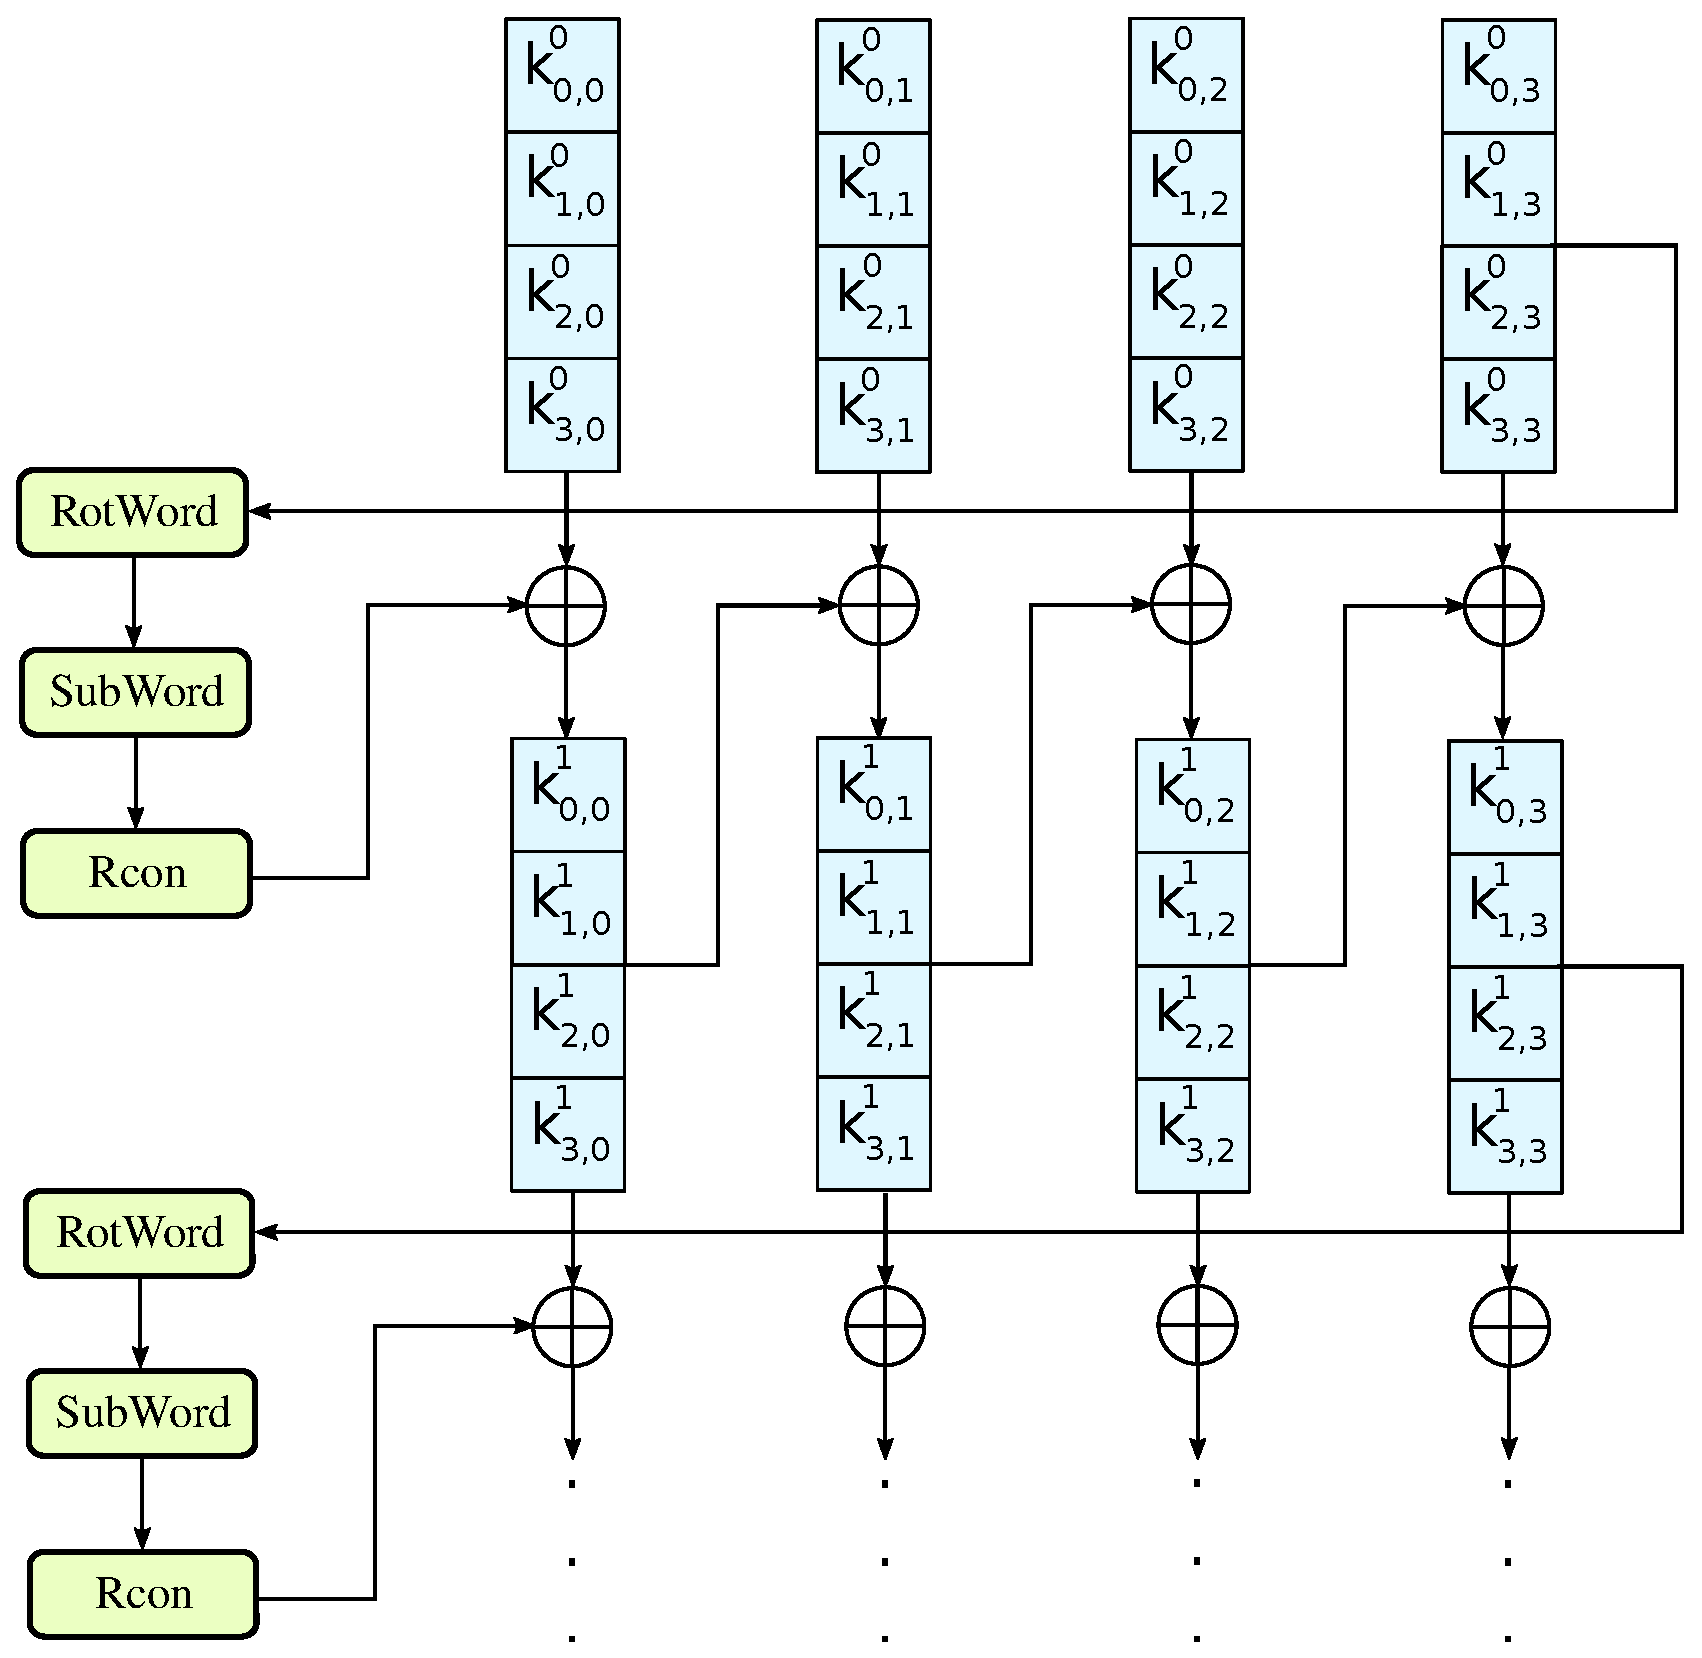
\includegraphics[scale=0.3]{images/aes-schedule.eps}
    \caption{AES key expansion}
    \label{aesschedule}
\end{figure}



\end{document}

